\chapter{きめつのやいば}\label{structure}

論文不知道寫什麼,去學一下呼吸型,寫論文就輕鬆了!

\section{日之呼吸}
學一下呼吸法阿$\sim$ \\
基本型有十二種,從千壽郎的書信中得知真正的型有十三種,炭治郎配戴的日輪花紙耳飾就是該呼吸法的繼承者之證。

\section{火之神神樂}
竈門家代代相傳的神事,其與「日之呼吸」有著深厚的關聯,使用者:竈門家族繼承者。

公式範例:
\begin{equation}
   \sqrt[n]{\frac{x^2+\sqrt 2}{x+y}}
\end{equation}

\begin{figure}
繪圖範例 1:\\[1em]
   \centering
      \pgfplotsset{width=6cm}          % 設置繪圖尺寸
      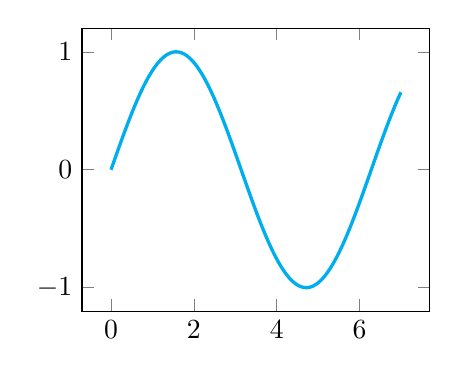
\begin{tikzpicture}
         \begin{axis}                  % 繪製座標
            % dashes = [10, 5, 100, 5] # 10 points on, 0 off, 100 on, 0 off
            \addplot [dash pattern=on 10 off 0 on 100 off 0, domain=0:7, samples=100, very thick, cyan] {sin(deg(x))};
         \end{axis}
      \end{tikzpicture}
   \caption{\edukai SIN FUNCTION}\label{fig:SIN FUNCTION}
\end{figure}
